%%%%%%%%%%%%%%%%%%%%%%%%%%%%%%%%%%%%%%%%%%%%%%%%%%%%%%%%%%%%%%%%%%%%%%%%%%%%%%%%%%%%%%%%%%%%%%%%%%%%%%%%%%%%%%%%%%%%%%%%
\newpage
\chapter {\Large{Setting Up Application}}


\section{Siminov Android ORM}


\begin{enumerate}

	\item \small Download Siminov Android ORM jar from \url{http://siminov.github.io/android-hybrid/builds.html}

	\item \small Add native orm jar into your application libs folder.

		\par
		\textbf{Example:} Siminov ORM Template Application
		\begin{figure}[htbp]
			\centering
				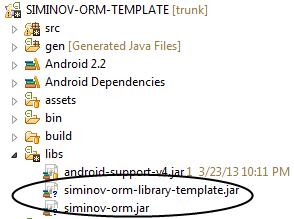
\includegraphics[height=8cm]{Resources/siminov_template_application_add_siminov_jar.png}
		\end{figure}	


\end{enumerate}




\section{Siminov Hybrid}

\begin{enumerate}

	\item \small Download Siminov Android ORM jar from \url{http://siminov.github.io/android-hybrid/builds.html}

	\item \small Download Siminov Hybrid build from \url{http://siminov.github.io/android-hybrid/builds.html}

	\item \small Extract Siminov Hybrid build into folder. 

		\par
		\textbf{Example:} Extract Siminov Build
		\begin{figure}[htbp]
			\centering
				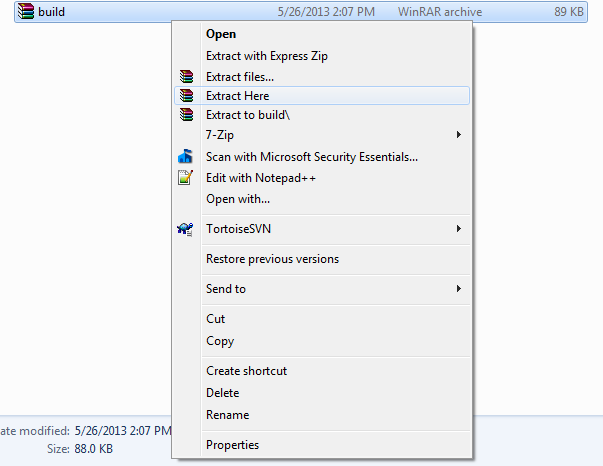
\includegraphics[height=8cm]{Resources/siminov_hybrid_build_extract.png}
		\end{figure}	

		\par
		\textbf{Example:} After Extracting Siminov Hybrid Build
		\begin{figure}[htbp]
			\centering
				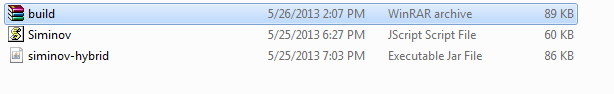
\includegraphics[height=2.5cm]{Resources/siminov_hybrid_build_extracted.png}
		\end{figure}	


	\newpage
	\item \small Add both native and hybrid jar's into your application libs folder.

		\par
		\textbf{Example:} Siminov Hybrid Template Application
		\begin{figure}[htbp]
			\centering
				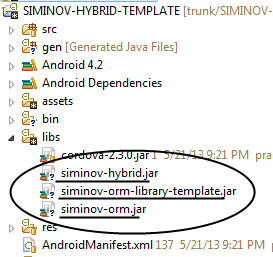
\includegraphics[height=6cm]{Resources/siminov_hybrid_template_application_add_siminov_jars.png}
		\end{figure}	


	\item \small Add Siminov JavaScript (Siminov.js) to your assets folder.
	
		\par
		\textbf{Example:} Siminov Hybrid Template Application
		\begin{figure}[htbp]
			\centering
				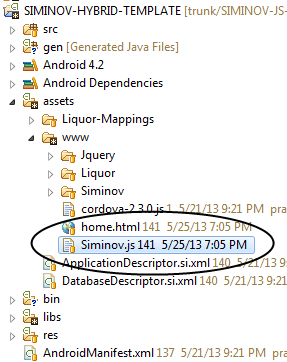
\includegraphics[height=8cm]{Resources/siminov_hybrid_template_application_add_siminov_js_to_application_assets.png}
		\end{figure}	
		

	\newpage
	\item \small Include Siminov JavaScript (Siminov.js) in your view.

		\par
		\textbf{Example:} Siminov Hybrid Template Application
		\begin{figure}[htbp]
			\centering
				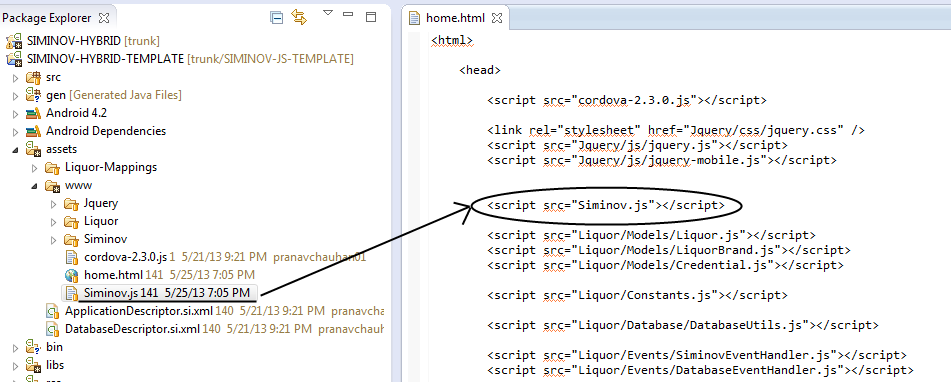
\includegraphics[height=7cm]{Resources/siminov_hybrid_template_application_include_siminov_js_to_application_view.png}
		\end{figure}	
		

	\item \small Invoke Siminov Initialization on device ready event.

		\lstinputlisting[language=Java]{Resources/siminov_hybrid_template_application_add_device_redy_event_listener_initialize_siminov.txt}


	\item \small Add Cordova Jar into your application libs folder.

		\par
		\textbf{Example:} Siminov Hybrid Template Application
		\begin{figure}[htbp]
			\centering
				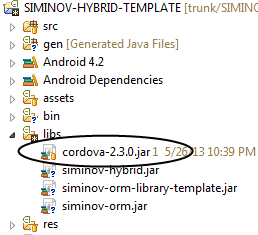
\includegraphics[height=5.5cm]{Resources/siminov_hybrid_template_application_add_cordova_jar.png}
		\end{figure}	
		

	\item \small Include Coredova JS file Into Your Project

		\par
		\textbf{Example:} Siminov Hybrid Template Application
		\begin{figure}[htbp]
			\centering
				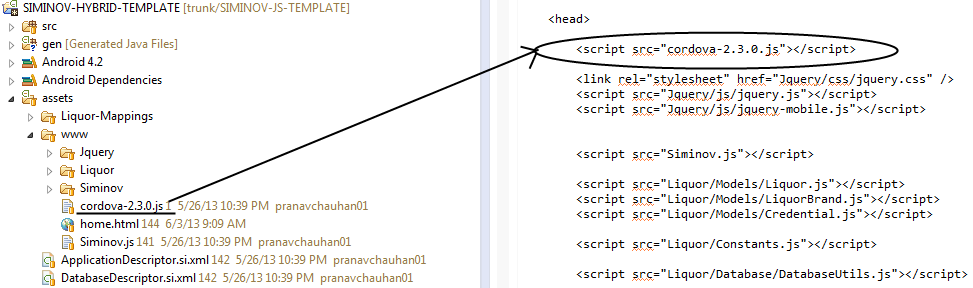
\includegraphics[height=5.2cm]{Resources/siminov_hybrid_template_application_include_cordova_into_project.png}
		\end{figure}	

	
\end{enumerate}
